\documentclass{article}

\usepackage[utf8x]{inputenc}
\usepackage[english,russian]{babel}
\usepackage{cmap}
\usepackage{commath}
\usepackage{amsmath}
\usepackage{amsfonts}
\usepackage{mathtools}
\usepackage{amssymb}
\usepackage{parskip}
\usepackage{titling}
\usepackage{color}
\usepackage{hyperref}
\usepackage{cancel}
\usepackage{enumerate}
\usepackage{multicol}
\usepackage{graphicx}
\usepackage[font=small,labelfont=bf]{caption}
\usepackage[a4paper, left=2.5cm, right=1.5cm, top=2.5cm, bottom=2.5cm]{geometry}

\graphicspath{ {./images/} }
\setlength{\droptitle}{-3cm}
\hypersetup{ colorlinks=true, linktoc=all, linkcolor=blue }
\pagenumbering{arabic}

\begin{document}
    \textbf{Пример.} Пусть \(x_1, x_2, x_3, ..., x_n\) --- произвольные положительные числа, причем \(x_1 x_2 x_3 ... x_n = 1\). Доказать, что \(x_1 + x_2 + ... + x_n \geq n\).

    \textbf{Определение.} \textit{Средним арифметическим} чисел \(a_1, a_2, a_3,..., a_n\) называется отношение \(\frac{a_1 + a_2 + ... + a_n}{n}\).

    \textbf{Определение.} \textit{Средним геометрическим} чисел \(a_1, a_2, a_3,..., a_n\) называется величина \(\sqrt[n]{a_1 a_2 ... a_n}\).

    \textbf{Теорема}(неравенство между средним арифметическим и средним геометрическим) \(\frac{a_1 + a_2 + ... + a_n}{n} \geq \sqrt[n]{a_1 a_2 ... a_n}\\ (\forall a_i > 0, i = 1, ..., n)\).

    \(\uparrow\) Это неравенство является следствием вышеупомянутого примера. Достаточно рассмотреть числа\\
    \(\frac{a_1}{\sqrt[n]{a_1 a_2 ... a_n}}, \frac{a_2}{\sqrt[n]{a_1 a_2 ... a_n}}, ..., \frac{a_n}{\sqrt[n]{a_1 a_2 ... a_n}}\)

    Их произведение равно 1 и они положительны, следовательно \(\frac{a_1}{\sqrt[n]{a_1 a_2 ... a_n}} + \frac{a_2}{\sqrt[n]{a_1 a_2 ... a_n}} + \frac{a_n}{\sqrt[n]{a_1 a_2 ... a_n}} \geq n \Rightarrow \frac{a_1 + a_2 + ... + a_n}{n} \geq \sqrt[n]{a_1 a_2 ... a_n} \downarrow\)

    \textbf{Замечание.} Знак равенства имеет место в неравенстве между средним арифметическим и средним геометрическим \(\Leftrightarrow a_1 = a_2 = a_3 = ... = a_n\).

    \subsection{Обобщение принципа математической индукции}

    Пусть \(p \in \mathbb{Z}\)(некоторое целое число). Предложение \(A(n)\), где \(n \in \mathbb{Z}\) истинно \(\forall n \geq p\), если выполнены следующие условия:
    \begin{enumerate}
        \item Предложение \(A(n)\) истинно при \(n = p\).
        \item Из истинности \(A(k)\ (k \in \mathbb{Z}, k \geq p) \Rightarrow\) что оно истинно при \(n = k+1\).
    \end{enumerate}
    \textbf{Пример.} Доказать, что любую сумму денег большую 7 рублей можно разменять только 3 и 5 рублёвыми монетами.
    \begin{enumerate}
        \item База индукции: \(8 = 3 + 5,\ 9 = 3 + 3 + 3,\ ...\)
        \item Пусть при \(n = k\) это возможно, т.е. \(k\) представимо в виде суммы 3-ек и 5-ок.
        \item Надо, что \(n = k + 1\) тоже представимо в виде суммы 3-ек и 5-ок
        
        Для \(k\) возможны два случая:

        \begin{enumerate}
            \item \(k\) --- сумма только 3-ек(их не меньше трёх, т.к. \(k \geq 8\)); тогда для \(k + 1,\ 3 + 3 + 3 + 1 = 5 + 5\)
            \item В разложение \(k\) есть 5-ка; тогда для \(k + 1,\ 5 + 1 = 3 + 3\)
        \end{enumerate}
    \end{enumerate}
    Из 1)-3) ч.т.д.

    \textbf{Пример.} Докажем неравенство между средним арифметическим и средним геометрическим ещё раз

    \(\frac{a_1 + a_2 + ... + a_n}{n} \geq \sqrt[n]{a_1 a_2 ... a_n} \quad (\frac{1}{n} \sum_{i = 1}^n a_i \geq \sqrt[n]{\Pi_{i=1}^n a_i},\ \ \forall a_i > 0,\ i = 1, ..., n)\)

    \begin{enumerate}
        \item \(n = 2 \quad \frac{a_1 + a_2}{2} \overset{?}{\geq} \sqrt{a_1 a_2}\)
        
        Действительно: \(\frac{a_1 + a_2}{2} - \sqrt{a_1 a_2} = \frac{a_1 - 2\sqrt{a_1 a_2} + a_2}{2} = \frac{(\sqrt{a_1} - \sqrt{a_2})^2}{2} \geq 0\)

        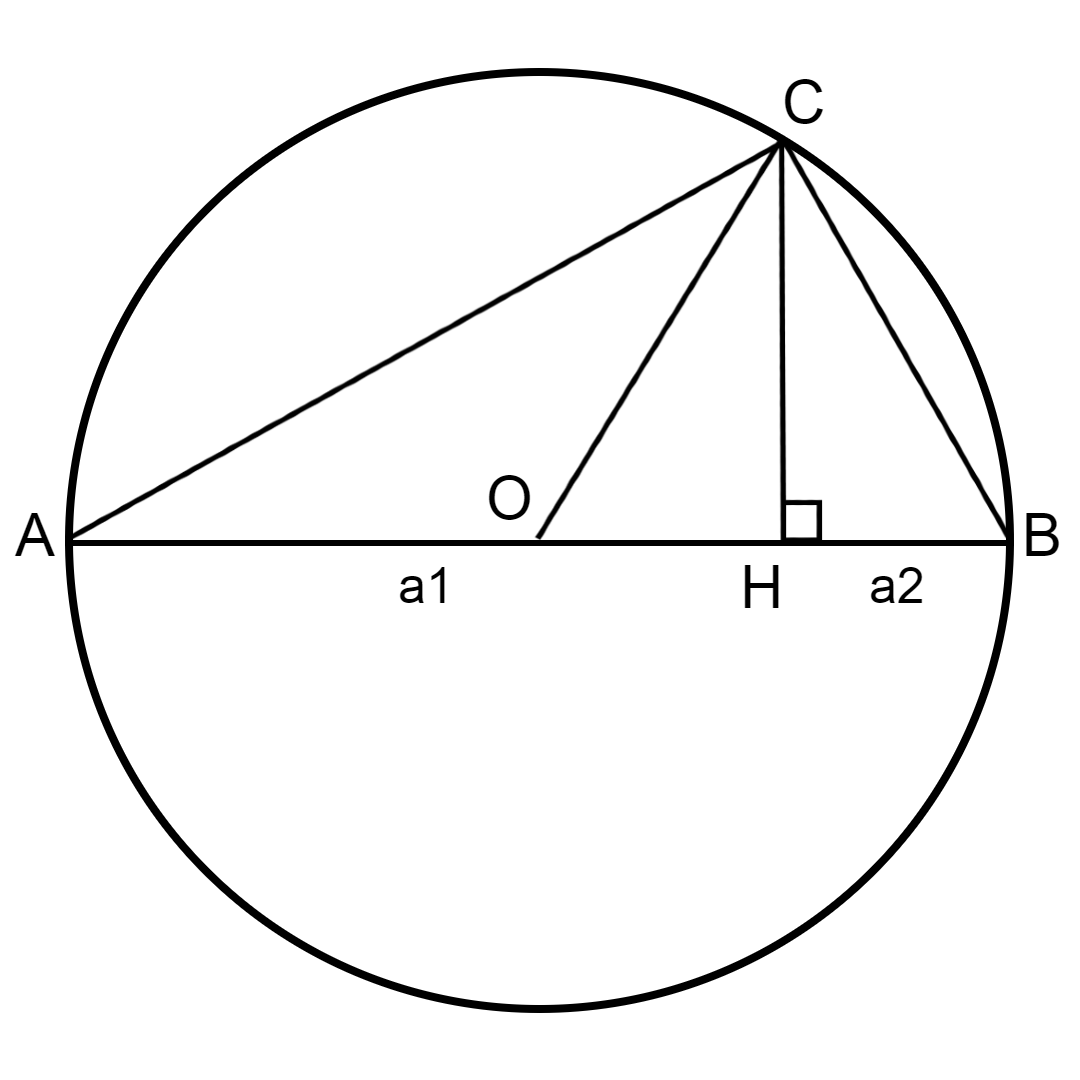
\includegraphics[scale=0.15]{9_1.png}
        \(AH=a_1, BH=a_2, AB\) --- диаметр окружности. В точке \(H\) восстановим перпендикуляр к \(AB\). \(C\) --- точка пересечения этого перпендикуляра с окружностью.

        \(CO=\frac{a_1 + a_2}{2}\) --- радиус окружности.

        \(CH = \sqrt{a_1 a_2} \quad (\frac{a_2}{CH} = \frac{CH}{a_1})\)

        В треугольнике гипотенуза больше катета. Равенство достигается, когда \(a_1 = a_2\). Ч.т.д.

        \item \(n = k\). Предположим, что выполнено \(\frac{a_1 + a_2 + ... + a_k}{k} \geq \sqrt[k]{a_1 a_2 ... a_k}\)\quad(**)
        
        \item \(n = 2k\). Доказать: \(\frac{a_1 + a_2 + ... + a_{2k}}{2k} \geq \sqrt[2k]{a_1 a_2 ... a_{2k}}\).
        
        \(\frac{a_1 + a_2 + ... + a_{2k}}{2k} = \frac{\frac{a_1 + a_2 + ... + a_k}{k} + \frac{a_{k+1} + ... + a_{2k}}{k}}{2} \overset{n-k}{\geq} \frac{\sqrt[k]{a_1 a_2 ... a_k} + \sqrt[k]{a_{k+1} ... a_{2k}}}{2} \overset{n-2}{\geq} \sqrt[2]{\sqrt[k]{a_1 a_2 ... a_k}\sqrt[k]{a_{k+1} a_{k+2} ... a_{2k}}} = \sqrt[2k]{a_1 a_2 ... a_{2k}}\)

        Таким образом, неравенство выполнено для всех \(n = 2^s(n=2,4,8,16,32...), s \in \mathbb{N}\).

        \item Если имеем утверждение для \(n=k\), докажем его при \(n=k-1\)(обратный ход).
        
        Надо доказать \(\frac{a_1 + a_2 + ... + a_{k-1}}{k-1} \geq \sqrt[k-1]{a_1 a_2 ... a_{k-1}}\).

        Рассмотрим (**) при \(a_k = \sqrt[k-1]{a_1 a_2 ... a_{k-1}}\). Имеем \(\frac{a_1 + a_2 + ... + a_{k-1} + \sqrt[k-1]{a_1 a_2 ... a_{k-1}}}{k} \geq\\ \sqrt[k]{a_1 a_2 ... a_{k-1} \sqrt[k-1]{a_1 a_2 ... a_{k-1}}} = (a_1 a_2 ... a_{k-1})^{(1 + \frac{1}{k-1})\frac{1}{k}} = (a_1 a_2 ... a_{k-1})^{\frac{1}{k-1}} = \sqrt[k-1]{a_1 a_2 ... a_{k-1}} \Leftrightarrow a_1 + a_2 + ... a_{k-1} + \sqrt[k-1]{a_1 a_2 ... a_{k-1}} \geq k\sqrt[k-1]{a_1 a_2 ... a_{k-1}} \Leftrightarrow a_1 + a_2 + ... a_{k-1} \geq (k-1)\sqrt[k-1]{a_1 a_2 ... a_{k-1}} \Leftrightarrow \frac{a_1 + a_2 + ... a_{k-1}}{k-1} \geq \sqrt[k-1]{a_1 a_2 ... a_{k-1}}\)

        Из 1)-4) ч.т.д.

        \textbf{Замечание.} Здесь важно, что \(\forall m \in \mathbb{N}\ \exists\ s : 2^s > m\)
    \end{enumerate}

    \section{Элементы комбинаторики}

    \textbf{Определение.} Если элементы множества как-либо пронумерованы, то говорят, что это множество \textit{упорядочено}.

    \textbf{Определение.} \textit{Декартовым(прямым) произведением} множества \(A\) на множество \(B\) называется множество всех упорядоченных пар \((a,b)\), где \(a \in A, b \in B\).
    \[A * B = \{(a,b), a \in A, b \in B\}\]
    \textbf{Пример.} Буквы азбуки Морзе состоят из символов точка и тире. Сколько букв в азбуке Морзе, если потребуем, чтобы каждая буква состояла не более чем из 5 указанных символов.

    Буква азбуки Морзе может состоять из одного символа, двух, трёх четырёх, пяти.
    \begin{enumerate}
        \item Односимвольных букв ровно 2: . и \(-\);
        \item Двухсимвольных:\quad\(\begin{aligned}
            &. \rightarrow \begin{aligned}
                &..\\
                &.-
            \end{aligned}\\
            &- \rightarrow \begin{aligned}
                &-.\\
                &--
            \end{aligned}\\
        \end{aligned}\quad 2 * 2 = 4\);
        \item Трёхсимвольных: \(4 * 2 = 8\);
        \item Четырёхсимвольных: \(8 * 2 = 16\);
        \item Пятисимвольных: \(16 * 2 = 32\).
    \end{enumerate}
    Итак, всего букв \(2+4+8+16+32=62\).

    \subsection{Основные правила комбинаторики}

    \begin{itemize}
        \item Правило суммы
        \item Правило произведения
    \end{itemize}

    \subsubsection{Правило суммы}
        
        Если элемент \(a\) можно выбрать \(n\) способами, а элемент \(b\) --- \(k\) способами, причём любой выбор элемента \(a\) отличен от любого выбора элемент \(b\), то выбор ``\(a\) или \(b\)'' можно осуществить \(n+k\) способами.
        
        \textbf{Утверждение.} Если пересечение конечных множеств \(A\) и \(B\) пусто \((A \cap B = \emptyset)\), то число элементов в их объединении равно сумме чисел элементов множеств \(A\) и \(B\).

        Если \((A \cap B = \emptyset)\), то \(m(A \cup B) = m(A) + m(B)\).

        \textbf{Следствие.} Если конечные множества \(A_1, A_2, ..., A_k\) попарно не пересекаются, т.е. при \(\forall i \not = j,\ A_i \cap A_j = \emptyset\), то имеет место равенство \(m(A_1 \cup A_2 \cup ... \cup A_k) = m(A_1) + m(A_2) + ... + m(A_k)\).

        \textbf{Утверждение.} Если задано отображение конечного множества \(X\) на множество \(Y\), то число элементов в \(X\) равно сумме чисел элементов в полных прообразах элементов множества \(Y\).

        \(\uparrow\) В самом деле, всё множество \(X\) распадается в этом случае на попарно непересекающиеся части --- полные прообразы элементов множества \(Y. \downarrow\)

    \subsubsection{Правило произведения}
        
        Если элемент \(a\) можно выбрать \(n\) способами и после каждого такого выбора элемент \(b\) можно выбрать другими \(k\) способами, то выбор ``\(a\) и \(b\)'' в указанном порядке можно осуществить \(n*k\) способами.

        \textbf{Утверждение.} Если множества \(A\) и \(B\) конечны, то число пар в их декартовом произведении \(A*B\) равно произведению чисел элементов этих множеств: \(m(A*B)=m(A)*m(B)\).

        \(\uparrow\) Декартово произведение множеств состоит из пар \((a, b)\), где \(a \in A, b \in B\). Если \(A = \{a_1, a_2, ..., a_n\}, B = \{b_1, b_2, ..., b_k\}\), то пары декартова произведения \(A*B\) можно записать в виде следующей таблицы:

        \((a_1, b_1), (a_1, b_2), ..., (a_1, b_k),\\
        (a_2, b_1), (a_2, b_2), ..., (a_2, b_k),\\
        ...\\
        (a_n, b_1), (a_n, b_2), ..., (a_n, b_k).\)

        В таблице \(n\) строк, \(k\) столбцов \(\Rightarrow\) всего элементов \(n*k. \downarrow\)

        \textbf{Следствие.} Если множества \(A_1, A_2, ..., A_s\) конечны, то имеет место равенство: \(m(A_1 * A_2 * ... * A_s) = m(A_1)*m(A_2)*...*m(A_s).\)

        \textbf{Утверждение.} Пусть задано отображение конечного множества \(X\) на множество \(Y\), причём в каждый элемент \(Y\) отображается одно и то же число элементов множества \(X\). Тогда число элементов во множестве \(X\) равно произведению числа элементов в \(Y\) на число элементов, отображающихся в элемент множества \(Y\).

        \(\uparrow\) Всё множество \(X\) распадается на попарно непересекающиеся части --- полные прообразы элементов множества \(Y\) при отображении. Поэтому число элементов в \(X\) равно сумме чисел во всех этих прообразах, а число полных прообразов равно числу элементов множества. По условию все прообразы имеют одинаковое число элементов. Поэтому
        \[m(X) = m(f^{-1}(b_1)) + m(f^{-1}(b_2)) + ... + m(f^{-1}(b_{m(Y)})) = m(f^{-1}(b_1)) * m(Y). \downarrow\]
\end{document}